%%%%%%%%%%%%%%%%%%%%%%%%%%%%% Define Article %%%%%%%%%%%%%%%%%%%%%%%%%%%%%%%%%%
\documentclass{article}
%%%%%%%%%%%%%%%%%%%%%%%%%%%%%%%%%%%%%%%%%%%%%%%%%%%%%%%%%%%%%%%%%%%%%%%%%%%%%%%

%%%%%%%%%%%%%%%%%%%%%%%%%%%%% Using Packages %%%%%%%%%%%%%%%%%%%%%%%%%%%%%%%%%%
\usepackage{geometry}
\usepackage{graphicx}
\usepackage{amssymb}
\usepackage{amsmath}
\usepackage{amsthm}
\usepackage{empheq}
\usepackage{mdframed}
\usepackage{booktabs}
\usepackage{lipsum}
\usepackage{graphicx}
\usepackage{color}
\usepackage{psfrag}
\usepackage{pgfplots}
\usepackage{bm}
\usepackage{babel}
\usepackage{biblatex}
%%%%%%%%%%%%%%%%%%%%%%%%%%%%%%%%%%%%%%%%%%%%%%%%%%%%%%%%%%%%%%%%%%%%%%%%%%%%%%%

% Other Settings

%%%%%%%%%%%%%%%%%%%%%%%%%% Page Setting %%%%%%%%%%%%%%%%%%%%%%%%%%%%%%%%%%%%%%%
\geometry{a4paper}
\graphicspath{{images/}}

%%%%%%%%%%%%%%%%%%%%%%%%%% Define some useful colors %%%%%%%%%%%%%%%%%%%%%%%%%%
\definecolor{ocre}{RGB}{243,102,25}
\definecolor{mygray}{RGB}{243,243,244}
\definecolor{deepGreen}{RGB}{26,111,0}
\definecolor{shallowGreen}{RGB}{235,255,255}
\definecolor{deepBlue}{RGB}{61,124,222}
\definecolor{shallowBlue}{RGB}{235,249,255}
%%%%%%%%%%%%%%%%%%%%%%%%%%%%%%%%%%%%%%%%%%%%%%%%%%%%%%%%%%%%%%%%%%%%%%%%%%%%%%%

%%%%%%%%%%%%%%%%%%%%%%%%%% Define an orangebox command %%%%%%%%%%%%%%%%%%%%%%%%
\newcommand\orangebox[1]{\fcolorbox{ocre}{mygray}{\hspace{1em}#1\hspace{1em}}}
%%%%%%%%%%%%%%%%%%%%%%%%%%%%%%%%%%%%%%%%%%%%%%%%%%%%%%%%%%%%%%%%%%%%%%%%%%%%%%%

%%%%%%%%%%%%%%%%%%%%%%%%%%%% English Environments %%%%%%%%%%%%%%%%%%%%%%%%%%%%%
\newtheoremstyle{mytheoremstyle}{3pt}{3pt}{\normalfont}{0cm}{\rmfamily\bfseries}{}{1em}{{\color{black}\thmname{#1}~\thmnumber{#2}}\thmnote{\,--\,#3}}
\newtheoremstyle{myproblemstyle}{3pt}{3pt}{\normalfont}{0cm}{\rmfamily\bfseries}{}{1em}{{\color{black}\thmname{#1}~\thmnumber{#2}}\thmnote{\,--\,#3}}
\theoremstyle{mytheoremstyle}
\newmdtheoremenv[linewidth=1pt,backgroundcolor=shallowGreen,linecolor=deepGreen,leftmargin=0pt,innerleftmargin=20pt,innerrightmargin=20pt,]{theorem}{Theorem}[section]
\theoremstyle{mytheoremstyle}
\newmdtheoremenv[linewidth=1pt,backgroundcolor=shallowBlue,linecolor=deepBlue,leftmargin=0pt,innerleftmargin=20pt,innerrightmargin=20pt,]{definition}{Definition}[section]
\theoremstyle{myproblemstyle}
\newmdtheoremenv[linecolor=black,leftmargin=0pt,innerleftmargin=10pt,innerrightmargin=10pt,]{problem}{Problem}[section]
%%%%%%%%%%%%%%%%%%%%%%%%%%%%%%%%%%%%%%%%%%%%%%%%%%%%%%%%%%%%%%%%%%%%%%%%%%%%%%%

%%%%%%%%%%%%%%%%%%%%%%%%%%%%%%% Plotting Settings %%%%%%%%%%%%%%%%%%%%%%%%%%%%%
\usepgfplotslibrary{colorbrewer}
\pgfplotsset{width=8cm,compat=1.9}
\setcounter{secnumdepth}{5}
\setcounter{tocdepth}{5}

\begin{document}
\begin{figure}[ht]
    \centerline{
\includegraphics[width=1.0\textwidth]{eFront_Logo.jpg}}
    \end{figure}
    \vspace*{1cm}
\begin{huge}
    \textbf{Report Technical Design Specification:}
\end{huge}
    \vspace{0.5cm}
    \begin{center}
    \begin{Huge}
    \textbf {Portfolio Review}
    \end{Huge}
    \end{center}
     \vspace*{2.0cm}
     \begin{center}
    \author{Documented by Ahuatzi RIOS}
    \end{center}
    \pagebreak
\titlepage
\tableofcontents
\newpage
\section{Business Requirements}
\label{sec:businessreq}
\lipsum[2]
\section{Report Structure and Requirements}
\label{sec:struc&req}
\lipsum[2]
\begin{figure}[ht]
    \centerline{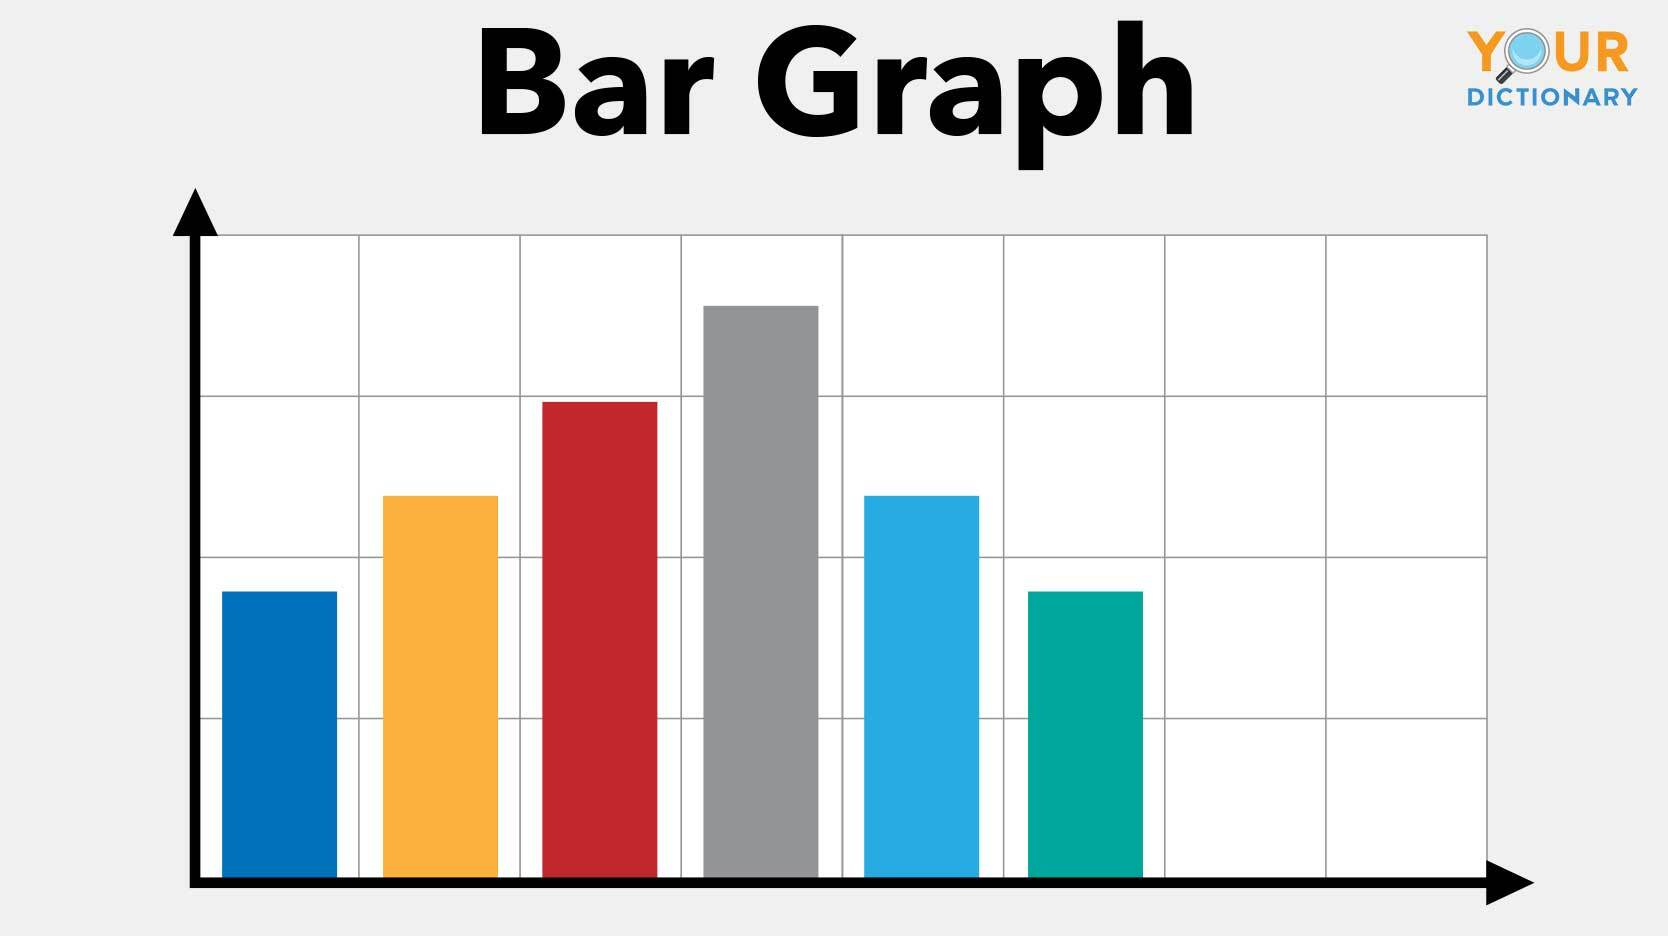
\includegraphics[width=1.0\textwidth]{bar-graph.jpg}}
    \end{figure}
    \pagebreak


\begin{huge}
\section{Calculations}
\label{sec:calcs}
\end{huge}
\subsection{Contributions}
\vspace*{1cm}
\textbf{The Contributions are represented by the Total Contributions amount from the consolidation of IF:QQ fund operations from all fund investments for the previous four years and YTD by using the formula:}
\[ Contributions = -Total Contributions\]
\begin{figure}[ht]
    \centerline{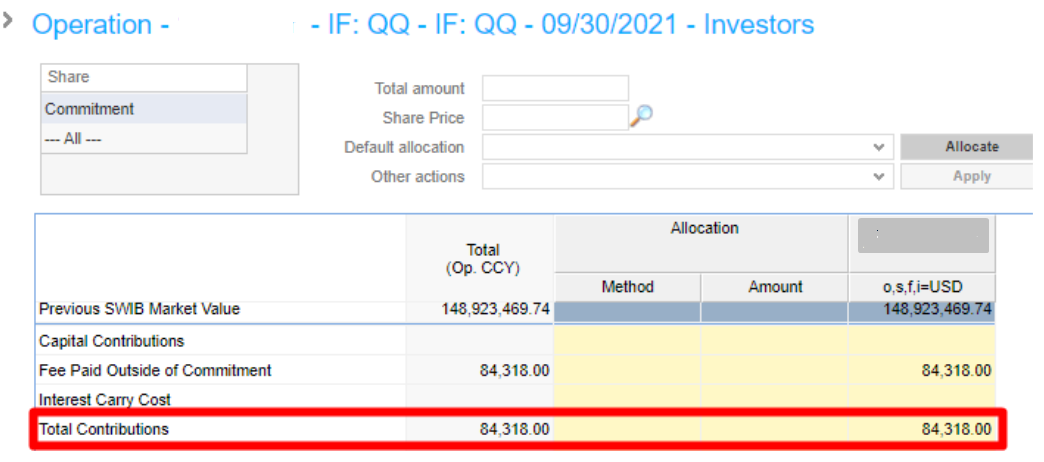
\includegraphics[width=1.0\textwidth]{contributions.png}}
    \end{figure}
\pagebreak
\subsection{Income}
\vspace*{1cm}
\textbf{The Income is represented by the Distributions of Income amount from the consolidation of IF:QQ fund operations from all fund investments for the previous four years and YTD: }
\begin{figure}[ht]
    \centerline{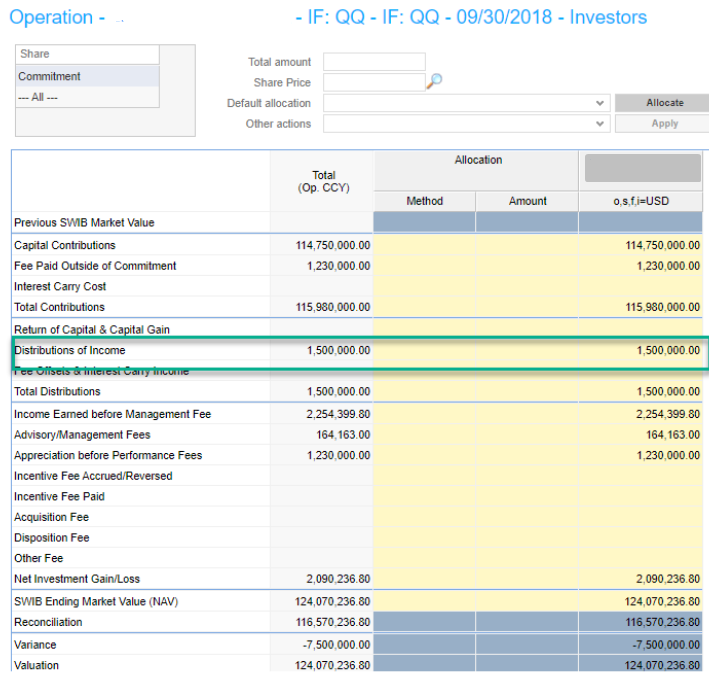
\includegraphics[width=1.0\textwidth]{income.png}}
    \end{figure}
\pagebreak
\subsection{Net Cash Flow}
\vspace*{1cm}
\textbf{The Income is represented by the Distributions of Income amount from the consolidation of IF:QQ fund operations from all fund investments for the previous four years and YTD: }
\[ Net Cash Flow = Contributions + Income + Return of Capital & Gain\]
\textbf{Code:}
\begin{verbatim}
    DATA WORK.T_PARTNERSHIP_SUMMARY;
    SET WORK.T_PARTNERSHIP_SUMMARY;

    TOTAL_GROSS_EXPOSURE=CONVERTCURR(TOTAL_GROSS_EXPOSURE,FUND_CURRENCY,"USD",ENTRY_DATE);
    NET_ASSET_VALUE=CONVERTCURR(NET_ASSET_VALUE,FUND_CURRENCY,"USD",ENTRY_DATE);
    CASH_CASH_EQUIVALENTS=CONVERTCURR(CASH_CASH_EQUIVALENTS,FUND_CURRENCY,"USD",ENTRY_DATE);

    SUBSCRIPTION_LINE_FINANCING=CONVERTCURR(SUBSCRIPTION_LINE_FINANCING,FUND_CURRENCY,"USD",ENTRY_DATE);
    TOTAL_FINANCE_BMTM=CONVERTCURR(TOTAL_FINANCE_BMTM,FUND_CURRENCY,"USD",ENTRY_DATE);
RUN;
\end{verbatim}

\end{document}